\documentclass[12pt]{article}
%\title{ Analyzing Radioactive Decay}
\title {Analyzing Radioactive Decay with Paremeter Estimation \\[1ex] \large Phsx 815- Project 3}

\author{Rakshak Adhikari}
\date{March 2021}
\usepackage{graphicx}
\usepackage{url}
\usepackage{amssymb}
\usepackage{subcaption} 
\usepackage{amsmath}
\usepackage{nicefrac}
\usepackage{xparse}
\begin{document}

\maketitle

\section{Introduction}	
This project involves analyzing counts over a fixed time from a radioactive substance, which will be distributed like a Poisson distribution. We will write a total likelihood function for the distribution and maximize it to get the best estimate for the lambda value. We will try this for several different values of lambda to properly explore the parameter space of the distribution. \\
We are especially interested in the results for small parameter values ($\lambda$) because that is where the distribution behaves differently than a normal distribution.\\
While the code is testing to identify Radioactive substance, the code can be used to test any Poisson Distribution for given lambda values.













\section{Theory}
Poisson distribution is characterized by the following equation.\begin{equation}\label{key}
P(x|\lambda)=\dfrac{exp(-\lambda)\lambda^x}{x!}
\end{equation}

Because we have n number of counts, we have n values for x and hence n functions of Lambda as our likelihood function. Our total likelihood then is simply the product of all those individual likelihood functions. 

\begin{equation}
\mathbb{L}_{total}=\Pi_{x=x_1}^{x_n}  \dfrac{exp(-\lambda)\lambda^x}{x!} 
\end{equation}
The factorials do not contribute when we are maximizing the function. So we define a reduced likelihood function that we use in the code denoted by: $\mathbb{L}$\\
\begin{equation}\label{key}
\mathbb{L}=\Pi_{x=x_1}^{x_n}  exp(-\lambda)\lambda^x=exp(-\lambda)\lambda^{\sum_{i=1}^{n}x_i}
\end{equation}

The second term in our expression may still be very large, so for optimization, it is much better to maximize the Log of the reduced likelihood function. We note that this is possible because our function is positive everywhere in the domain.\\
\begin{equation}\label{key}
Log(\mathbb{L})= -n\lambda+ln(x)\sum_{0}^{n}x_i
\end{equation}















%
%
%
%
\section{Algorithm}
\paragraph{Simulating the Decay:}
Simulator.py simulates the radioactive decay using the python standard P
oisson distribution generator. A series of lambda values is supplied as input and a distribution is outputted for each lambda values supplied. The number of measurements is also supplied.
For the run, the following values were used:
\begin{center}

	$\lambda=[2,3,4,5,10,25,50,100]$\\

	no of experiments =$10^5$ \\
	no of measurements per experiment= 1\\	
	
\end{center}
 \begin{figure}[h!]
	
	
	
	\begin{subfigure}[h!]{0.8\textwidth}
		\centering
		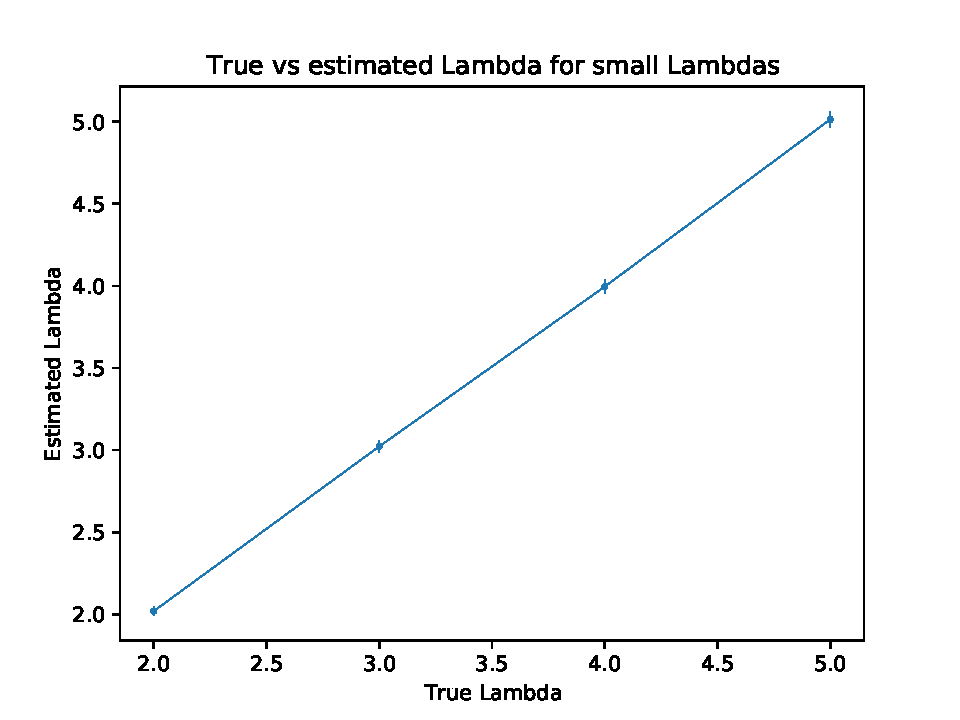
\includegraphics[width=\textwidth]{fig1.pdf}
		\caption{Small $\lambda$}
		
	\end{subfigure}
	
	\begin{subfigure}[h!]{0.8\textwidth}
		\centering
		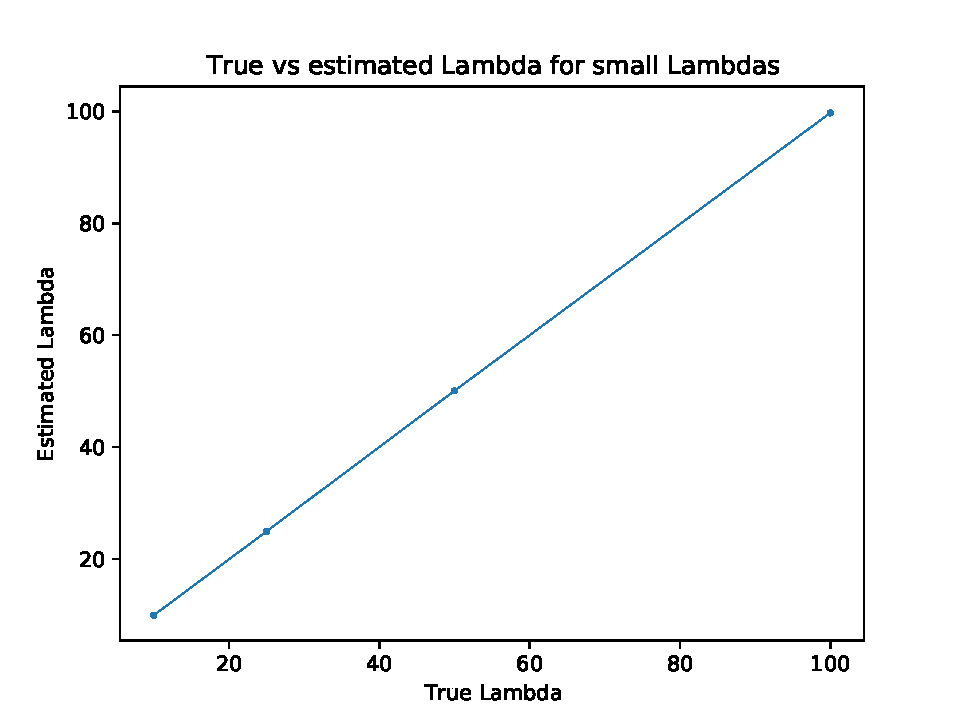
\includegraphics[width=\textwidth]{fig2.pdf}
		\caption{Large $\lambda$}
		
	\end{subfigure}	
\end{figure}

\paragraph{Analyzing the Output:}
$Parameterestimator.py$ uses the scipy.optimize function
 to minimize the negative log likelihood function for each dataset.\\
It reads all the output text files produced by simulator.py and calculates the Likelihood function for each of the parameter values and maximizes the likelihood. It then outputs the maximized parameter value as well as the variance of the estimate. The glob function is used to read all the text files iteratively and matplotlib is used to plot.

\vspace{0.5cm}







\section{Result}
Since we wanted to probe for smaller values of Lambda where the Poisson distribution does not resemble a gaussian, we ran the script in two batches: one for smaller values of lambda and one for larger values of lambda. This allowed us to see the five sigma uncertainty which was small and was not visible if we had plotted all of the data together.

The errors were very small and are tabulated below:
\begin{center}
	\begin{tabular}{||c c c c||} 
		\hline
		True Lambda & Estimated Lambda & 5-Sigma  \\ [0.5ex] 
		\hline\hline
		2 & 2.0202 & 0.0275  \\ 
		\hline
		3 & 3.0227 & 0.0389  \\
		\hline
		4 & 3.9954 & 0.0446  \\
		\hline
		5 & 5.0132 & 0.0481  \\
		\hline
		10 & 9.9483 & 0.0704  \\
		\hline
		25 & 24.9339 & 0.1107  \\
		\hline
		50 & 50.0492 & 0.1585 \\
		\hline
		100 & 99.7173 & 0.2409  \\[1ex]
		\hline
		 

	\end{tabular}
\end{center}


	
\section{Conclusion}
The rate parameter can be estimated using minimization of the total likelihood function.
	
	
	
	
\begin{thebibliography}{9}
	\bibitem{DecaySimulator}
	\url{https://github.com/Raxxak/PHSX815_Project3/blob/main/simulator.py} 
	\bibitem{Decay analysis Lik} 

	\url{https://github.com/Raxxak/PHSX815_Project2/blob/main/ParameterEstimator.py}
	

	
\end{thebibliography}
	
\end{document}